\section{Evaluation}
\label{sec:eval}

We evaluate the benefits of our implementation on our micro-benchmark (described
above) across a range of parameters. We implement the compression algorithm in
the last level of cache. The metrics used for evaluation are the miss rate in
the last level of cache in MPKI and the effective cache capacity increase or
Effective Compression Ratio (ECR) which measures the compressibility of the data
that can actually be utilized with the limitations of hardware implementation.
Figure~\ref{fig:size} shows the benefits of the splitting optimization for different data
set sizes. The miss rate increases with the data set size and the difference in
miss rates between the split vs unsplit structures increases with the size of
the working and stabilizes at higher sizes.  

\begin{figure}[htb]
\centering
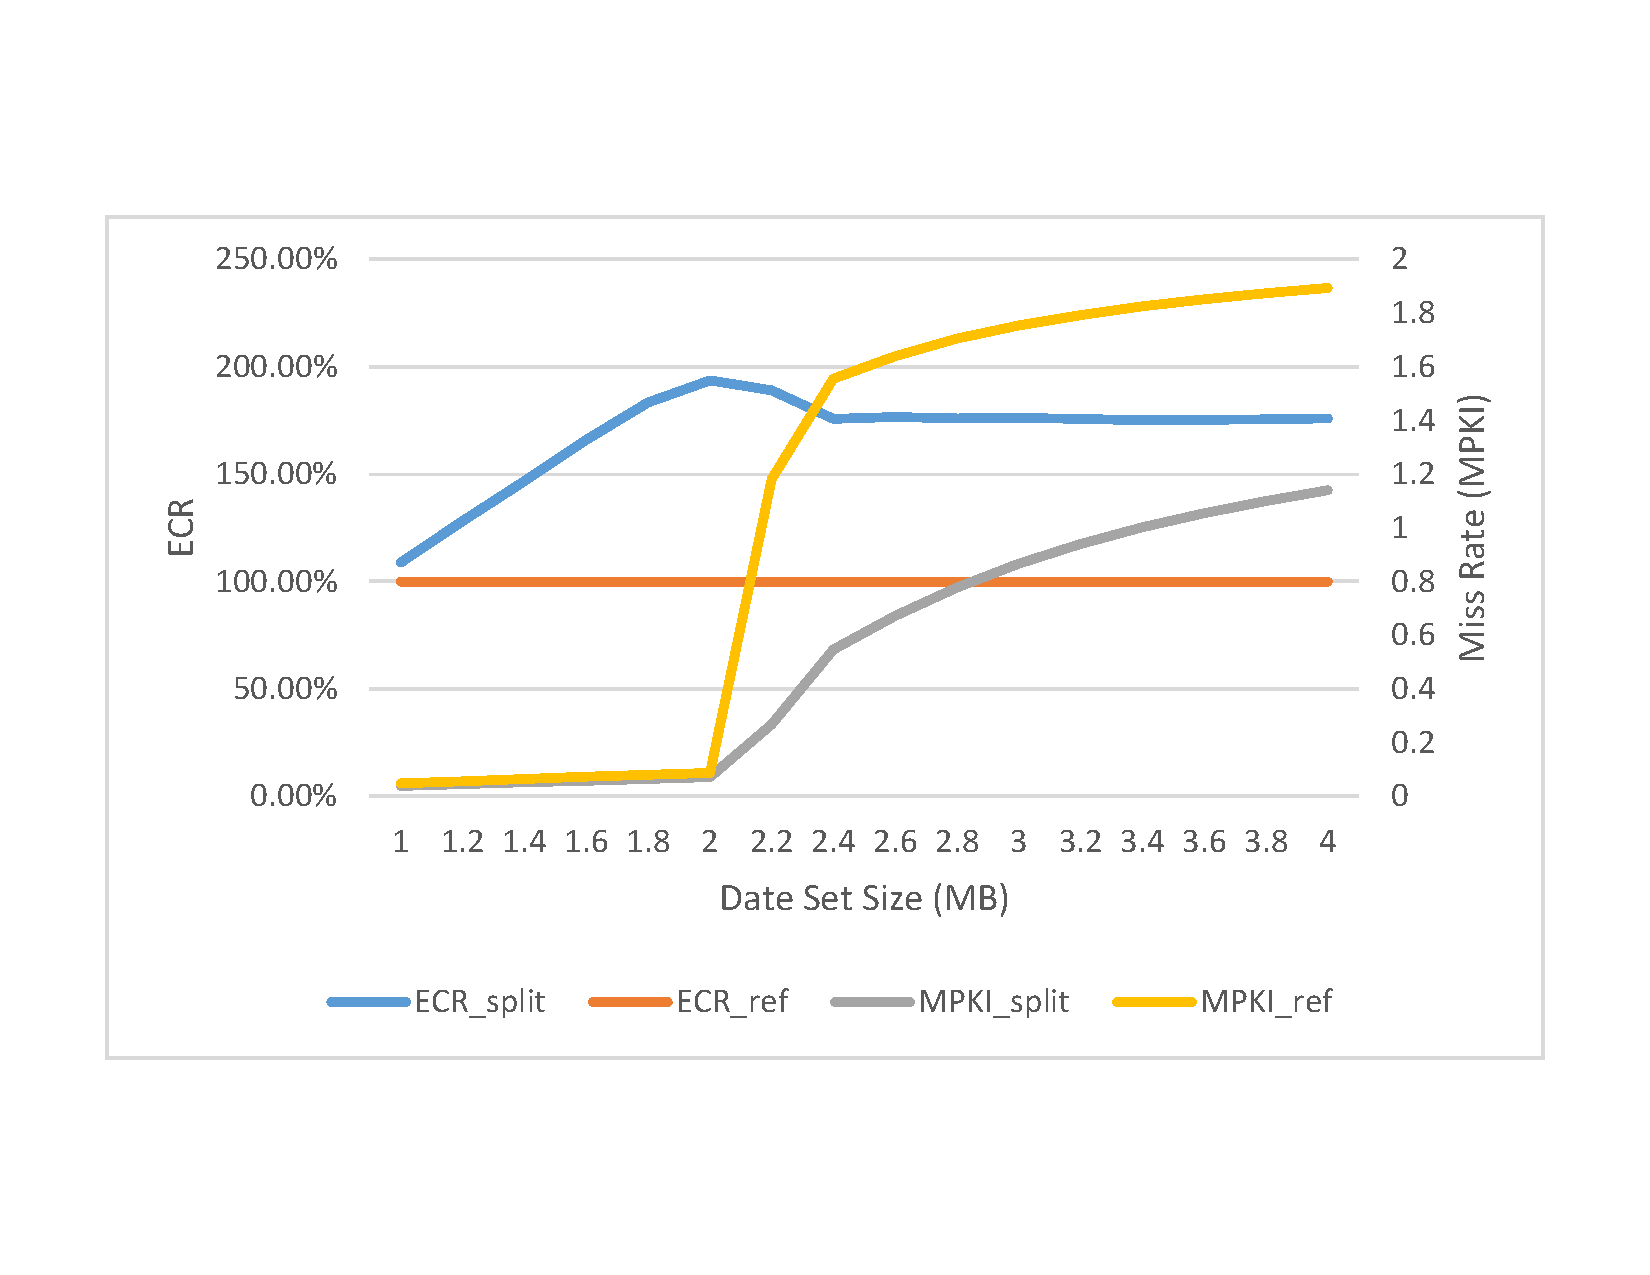
\includegraphics[trim=0mm 0mm 0mm 0mm,clip,width=1\linewidth]{figs/figure2.pdf}
\caption{Effective compression ratio and cache misses per kilo-instructions when
varying the data set size.}
\label{fig:size}
\end{figure}

The splitting benefit for different field affinities is depicted in
Figure~\ref{fig:affinity}.  Here we vary the probability that two fields are
accessed together. In this case we use a random access pattern. There is no
change in compressibility, as expected. As the affinity between the two fields
increases, the miss rate increases when data splitting is employed. This is
because, the benefits from locality outweigh the compression benefits for all
cases except when there is little or no affinity between the fields. The effect
is further exacerbated by the lack of reuse in the data since the access pattern
is random. Figure~\ref{fig:range} shows the variation in compressibility with
differing dynamic ranges. And finally, we evaluate the impact of our
optimization for different field types. We use different combinations of char,
int, float and pointer and illustrate the difference in compressibility and
cache utilization when using data splitting across different field types.
Figure~\ref{fig:type} shows that the impact of data splitting is greatest with
disparate data fields like pointer and char types in the same data structure.
Table~\ref{tbl:field-combinations} maps the different data points in the graph
to the corresponding field combinations. 

\begin{figure}[htb]
\centering
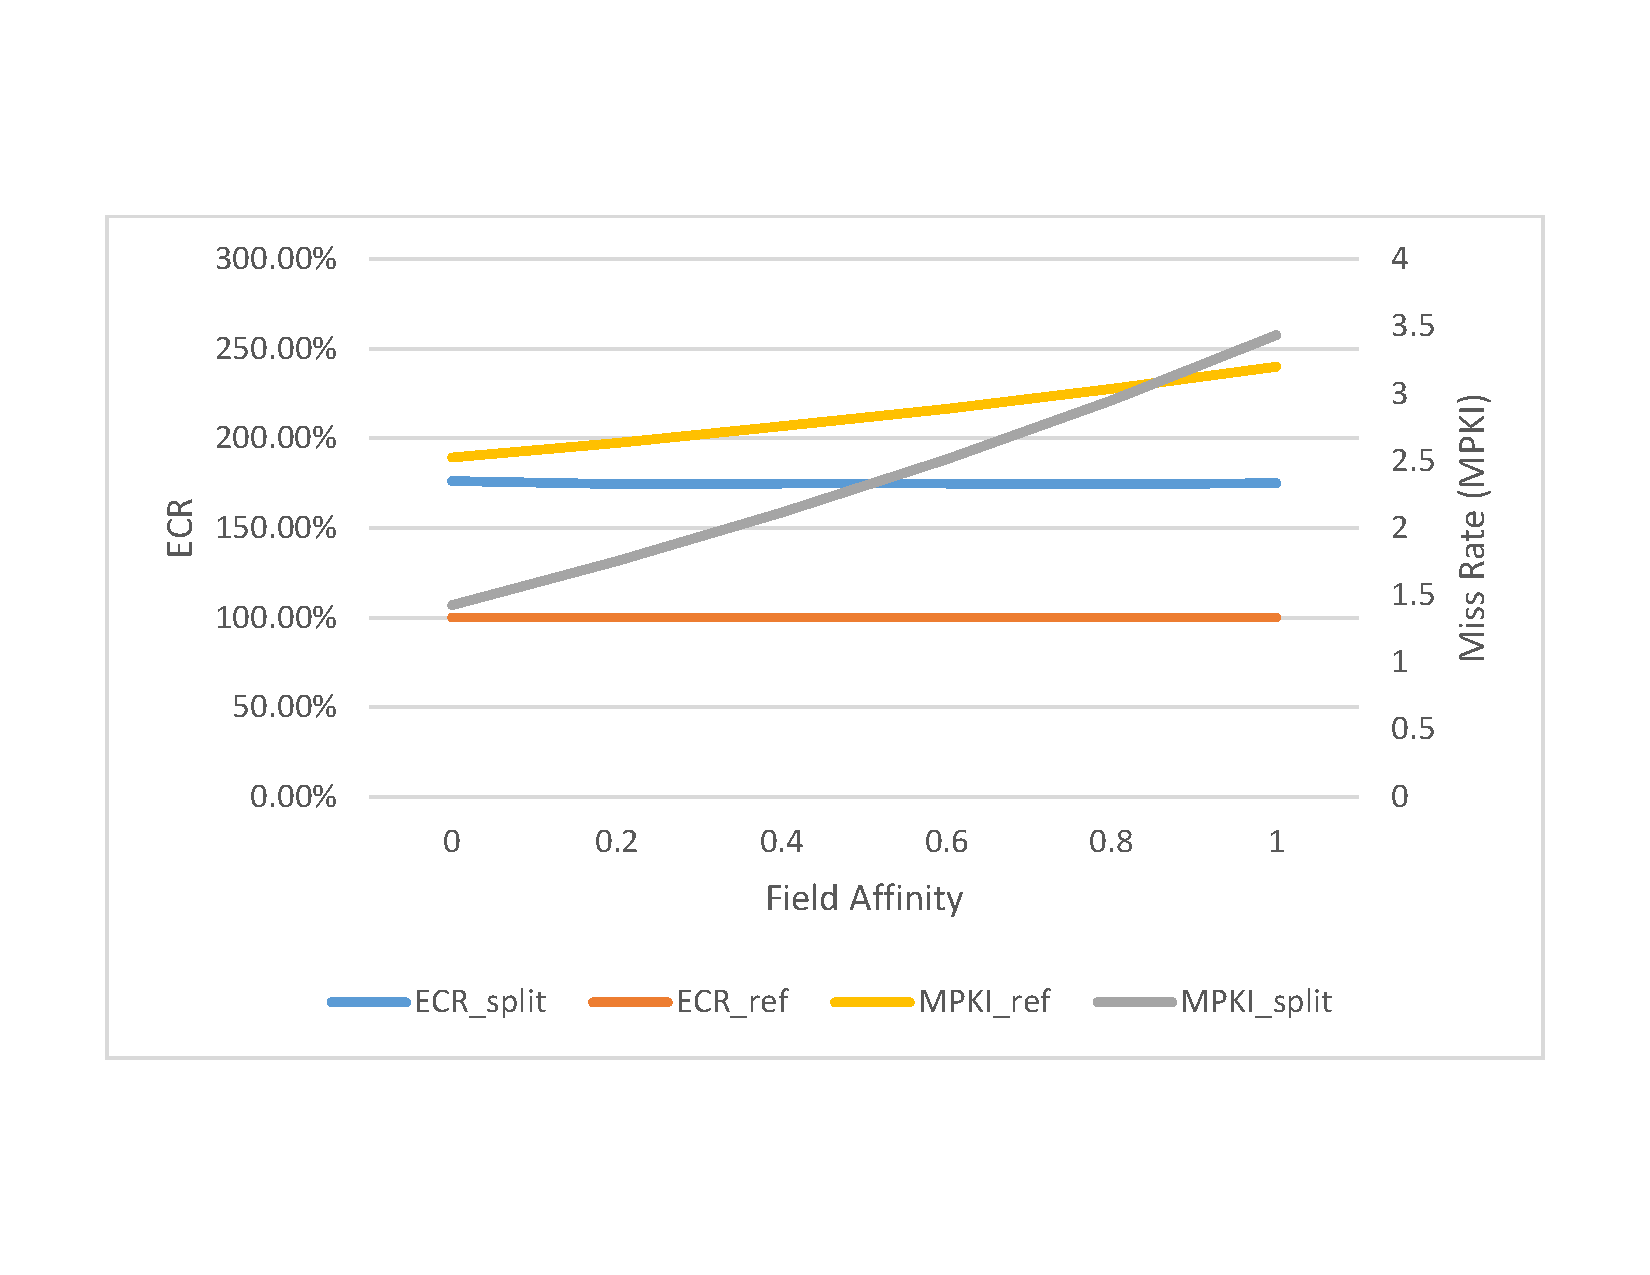
\includegraphics[trim=0mm 0mm 0mm 0mm,clip,width=1\linewidth]{figs/figure.pdf}
\caption{Effective compression ratio and cache misses per kilo-instructions when
varying the affinity value.}
\label{fig:affinity}
\end{figure}

\begin{figure}[htb]
\centering
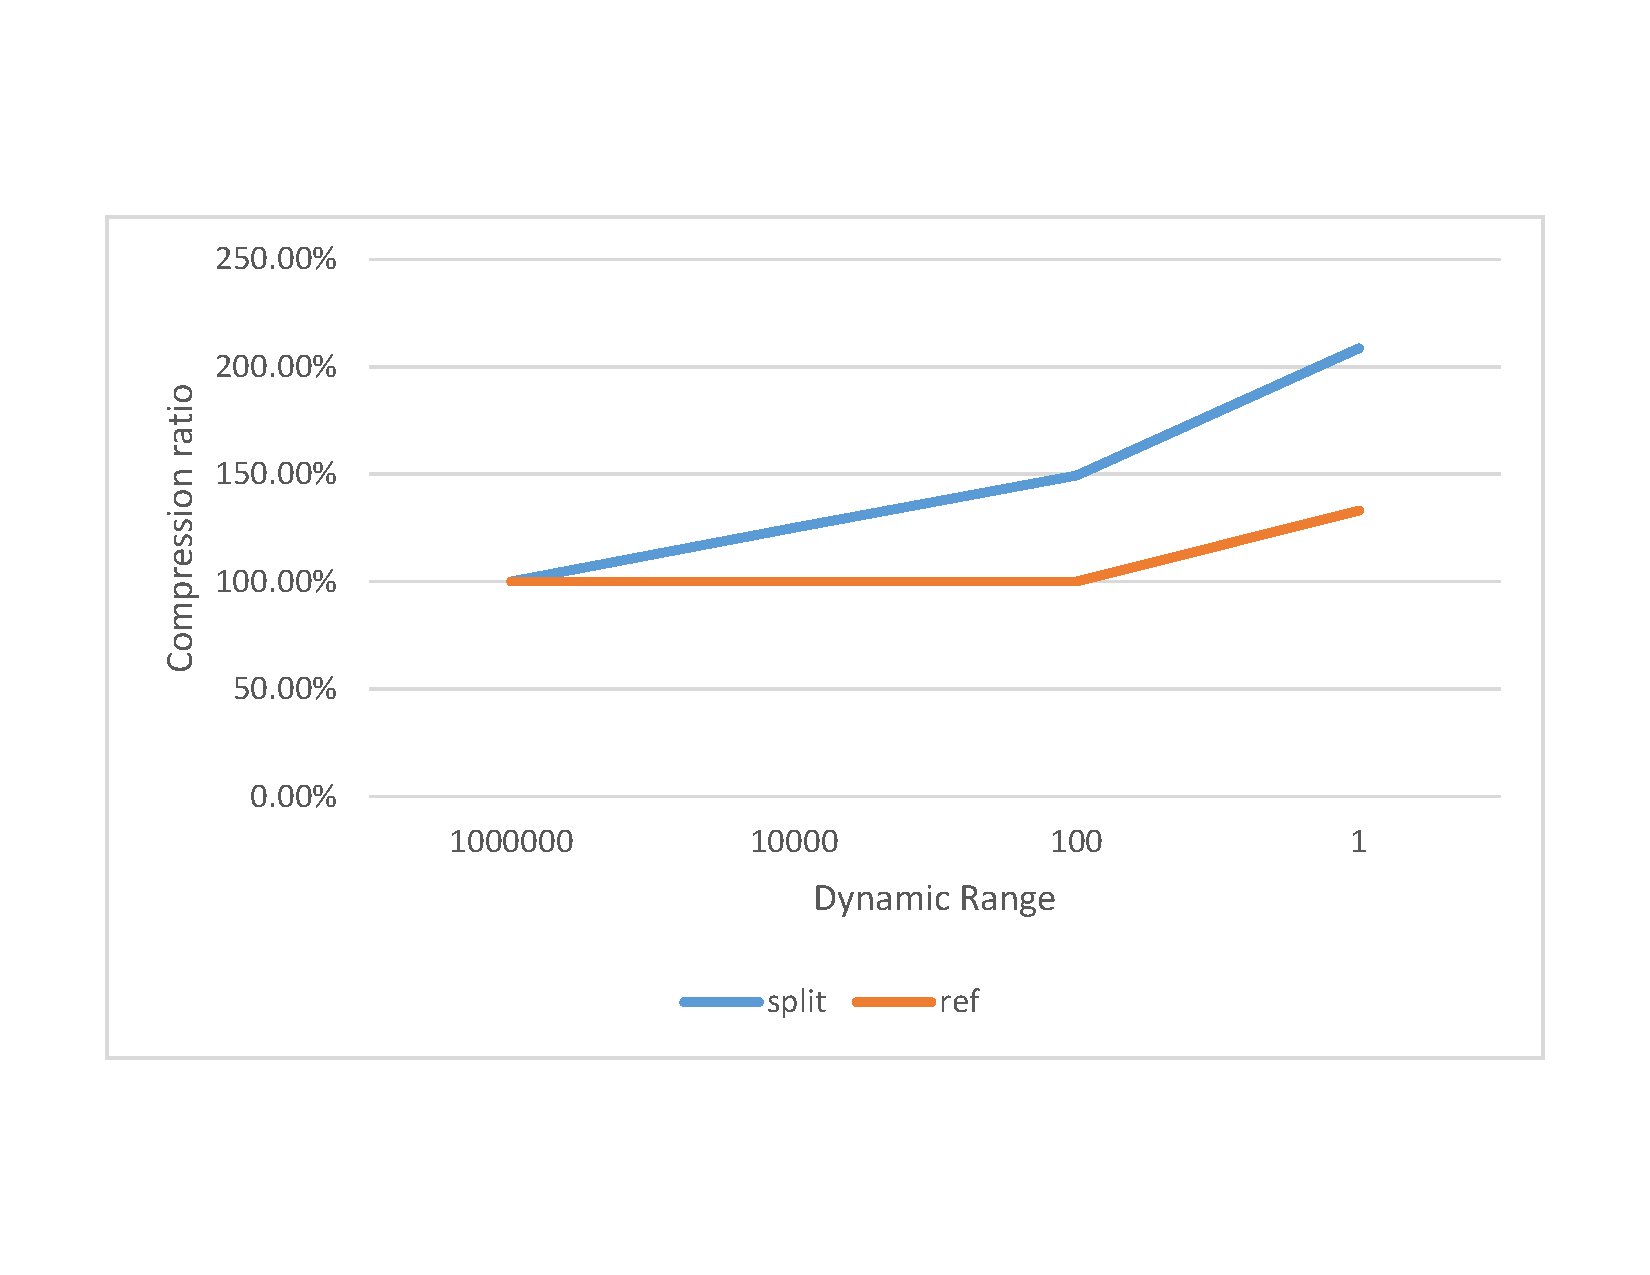
\includegraphics[trim=0mm 0mm 0mm 0mm,clip,width=1\linewidth]{figs/figure3.pdf}
\caption{Effective compression ratio and cache misses per kilo-instructions when
varying the dynamic range.}
\label{fig:range}
\end{figure}

\begin{figure}[htb]
\centering
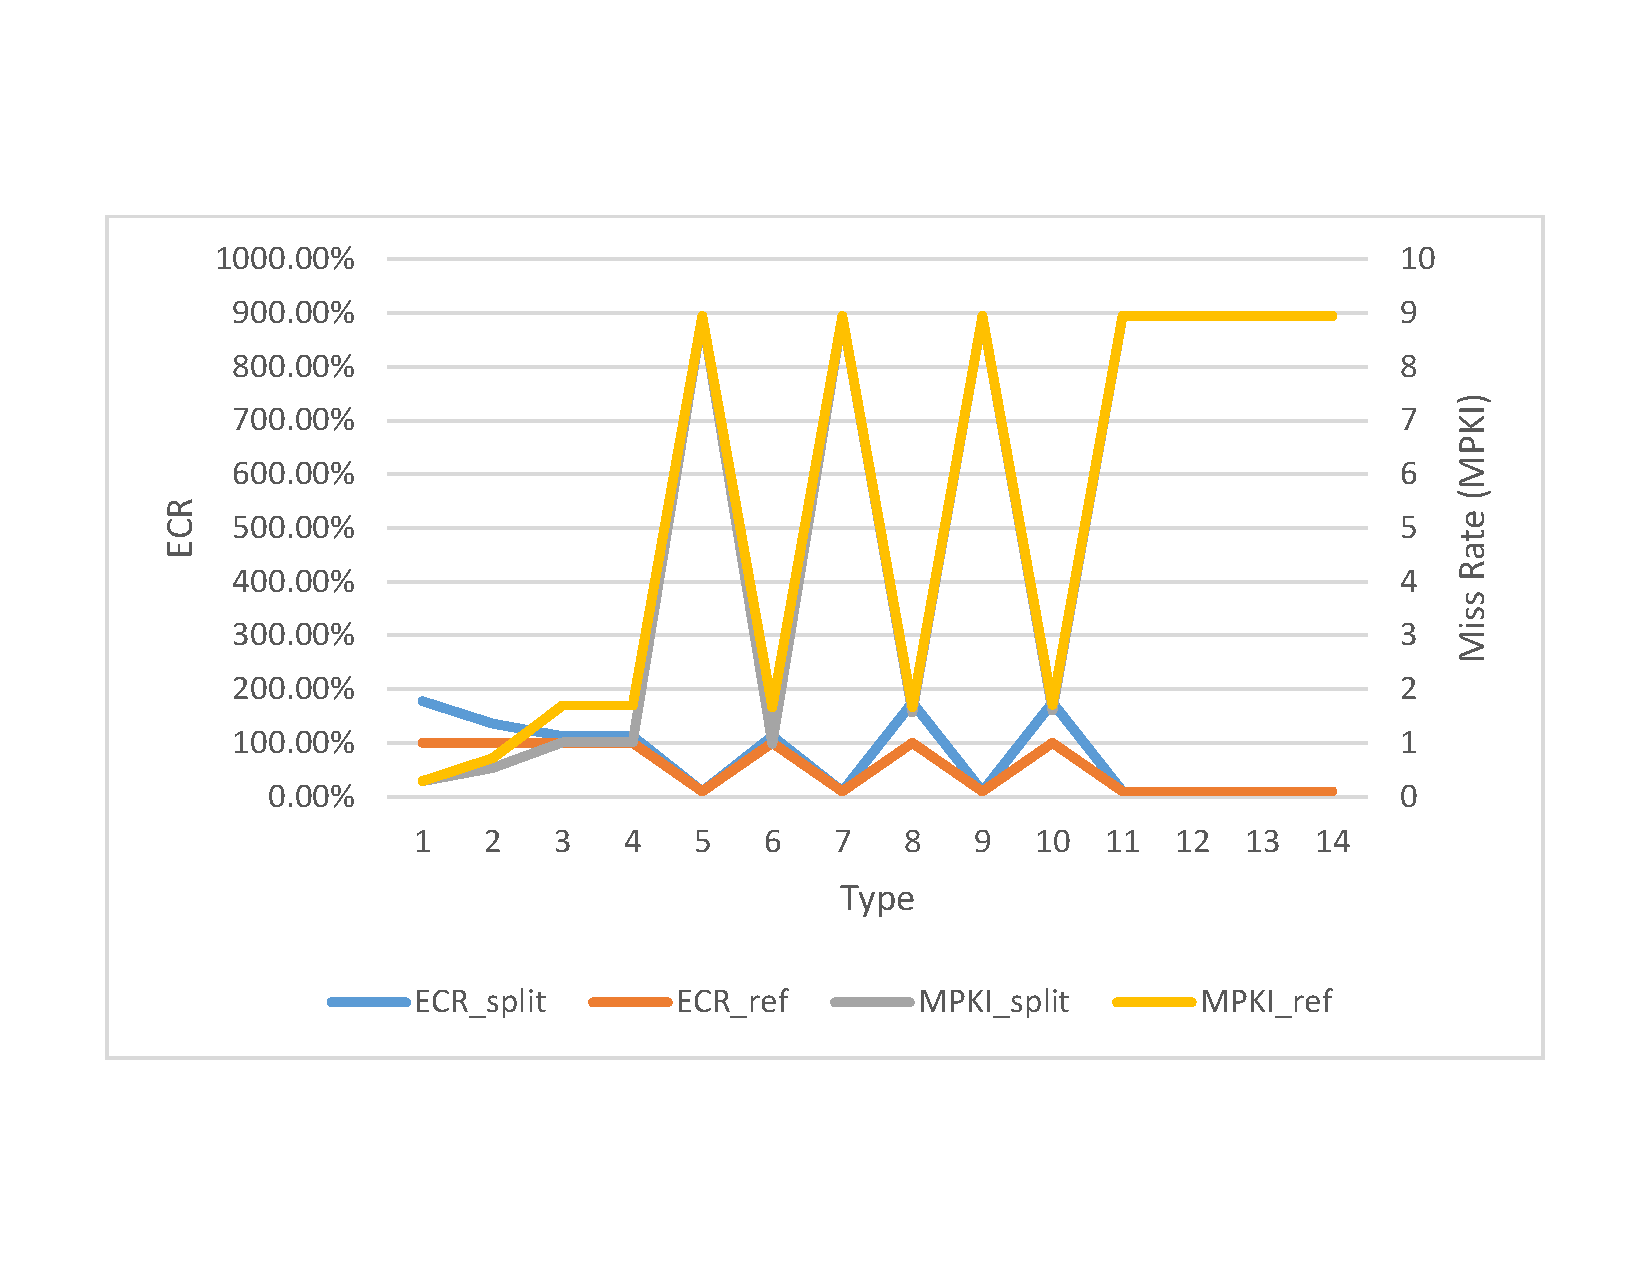
\includegraphics[trim=0mm 0mm 0mm 0mm,clip,width=1\linewidth]{figs/figure4.pdf}
\caption{Effective compression ratio and cache misses per kilo-instructions when
varying the field types.}
\label{fig:type}
\end{figure}

\begin{table}[htb]
\centering
\begin{tabular}{ccc}
\toprule
Label & Field 1 type & Field 2 type \\
\midrule
1 & char & char \\
2 & char & short \\
3 & char & int* \\
4 & char & int \\
5 & char & long long \\
6 & char & float \\
7 & char & double \\
8 & int & float \\
9 & int & double \\
10 & int & int* \\
11 & float & double \\
12 & long long & double \\
13 & long long & float \\
14 & long long & int \\
\bottomrule
\end{tabular}
\caption{Field types combinations.}
\label{tbl:field-combinations}
\end{table}

